
%% HUH Colloquium Presentation
%% Tom Eichlersmith

\documentclass{beamer}

\mode<presentation> {
	\usetheme{Goettingen}
	\setbeamertemplate{navigation symbols}{}
	\setbeamertemplate{footline}[page number]
}

\usepackage{graphicx} % Allows including images
\usepackage{booktabs} % Allows the use of \toprule, \midrule and \bottomrule in tables
\usepackage{subfigure} % For images next to each other

%-----------------------------------------------
%%	TITLE PAGE
%-----------------------------------------------

\title[Random Walks]{Random Walks on Simple Two-Dimensional Manifolds} % The short title appears at the bottom of every slide, the full title is only on the title page

\author{Tom Eichlersmith}
\institute[Hamline U]
{
Hamline University \\
\medskip
\texttt{teichlersmith01@hamline.edu}
}
\date{\today}

\begin{document}

\begin{frame}
	\titlepage % Print the title page as the first slide
\end{frame}

\begin{frame}
	\frametitle{Overview} % Table of contents slide, comment this block out to remove it
	\tableofcontents % Throughout your presentation, if you choose to use \section{} and \subsection{} commands, these will automatically be printed on this slide as an overview of your presentation
\end{frame}

%------------------------------------------------
%%	PRESENTATION SLIDES
%------------------------------------------------

\section{Introduction} 

\begin{frame}

	\frametitle{Introduction}
	
	\begin{itemize}
		\item Random
		\item Walk
		\item Simple
		\item Two-Dimensional
		\item Manifolds
	\end{itemize}

\end{frame}

%------------------------------------------------
\section{Background}

\begin{frame}

	\frametitle{Regular Surfaces}
	
	\textit{Coordinate Patch} $\mu:U\to V$ : continuous functions mapping from $U\subseteq\mathbb{R}^2$ to a subset of the surface $V$
	
	\vskip 2em
	
	\textit{Chart} : covers entire surface
	
	\vskip 2em
	
	Regular Surfaces:
	\begin{itemize}
		\item Differentiable --- the coordinate functions of $\mu$ in $\mathbb{R}^3$ have continuous partial derivatives for all orders
		\item Homeomorphic --- $\mu$ and its inverse are continuous
		\item Satisfies the Regularity Condition --- The differential of $\mu$ is a one-to-one linear transformation
	\end{itemize}

\end{frame}

%---------------------------------------------------------------

\begin{frame}
	
	\frametitle{Charts}

	\begin{align*}
	\phi:&\mathbb{R}^2 \to P\\
	\phi(u,v) &= (u,v,0)
	\end{align*}
	
\end{frame}

%---------------------------------------------------------------

\begin{frame}
	
	\frametitle{Charts}
	
	\begin{align*}
	\sigma:&\mathbb{R}^2 \to S \\
	\sigma(u,v) &= \left(\frac{2u}{1+u^2+v^2},\frac{2v}{1+u^2+v^2},\frac{-1+u^2+v^2}{1+u^2+v^2}\right)
	\end{align*}
	
\end{frame}

%---------------------------------------------------------------

\begin{frame}
	
	\frametitle{Charts}
	
	\begin{align*}
	\tau:&[0,1)\times[0,1) \to T(R,r) \\
	\tau(u,v) = \Big(&(R+r\cos(2\pi v))\cos(2\pi u), \\
	&(R+r\cos(2\pi v))\sin(2\pi u), \\
	&r\sin(2\pi v) \Big)
	\end{align*}
	
\end{frame}

%---------------------------------------------------------------

\begin{frame}
	
	\frametitle{Geodesic Equations}
	
	\begin{enumerate}
		\item Extend definition of line to other surfaces
		\item Assume a path is a geodesic contained in a coordinate patch
		\item Derive geodesic equations for coordinate functions of path
	\end{enumerate}

\end{frame}

%---------------------------------------------------------------

\begin{frame}
	
	\frametitle{Geodesic Equations}
	
	\begin{align*}
		u'' + \frac{\mu_{uu} \cdot \mu_u}{\mu_u \cdot \mu_u} (u')^2 + \frac{\mu_{vv} \cdot \mu_u}{\mu_u \cdot \mu_u} (v')^2 + 2\frac{\mu_{uv} \cdot \mu_u}{\mu_u \cdot \mu_u} u'v' & = 0 \\
		v'' + \frac{\mu_{uu} \cdot \mu_v}{\mu_v \cdot \mu_v} (u')^2 + \frac{\mu_{vv} \cdot \mu_v}{\mu_v \cdot \mu_v} (v')^2 + 2\frac{\mu_{uv} \cdot \mu_v}{\mu_v \cdot \mu_v} u'v' & = 0 \\
	\end{align*}
	
	
\end{frame}

%---------------------------------------------------------------

\begin{frame}
	
	\frametitle{Christoffel Symbols}
	
	\begin{equation*} 
		\Gamma^i_{jk} = \frac{\mu_{jk}\cdot\mu_i}{\mu_i\cdot\mu_i} \quad\text{where } i,j,k \in \{u,v\}
	\end{equation*}
	
	$$\Big\Downarrow \text{abuse of symbols}$$
	
	\begin{equation*}
		\frac{d^2x^i}{dt^2} + \sum_{j,k \in \{1,2\}} \Gamma^i_{jk}\frac{dx^j}{dt}\frac{dx^k}{dt} = 0
	\end{equation*}
	
\end{frame}

%------------------------------------------------
\section{Method}

\begin{frame}

	\frametitle{Stepping Method}
	
	Runge-Kutta 4th Order Method (RK4)
	\begin{equation*}
		\frac{dy}{dt} = F(y) \quad y_0 = y(0)
	\end{equation*}
	Numerically solve up to $t=h$ with $N$ iterations.
	\begin{align*}
		& \delta \gets h/N \\
		& y \gets y_0 \\
		& \textit{loop } N \textit{ times:} \\
		& \quad\quad k_1 \gets F(y) \\
		& \quad\quad k_2 \gets F\left(y+(\delta/2)k_1\right) \\
		& \quad\quad k_3 \gets F\left(y+(\delta/2)k_2\right) \\
		& \quad\quad k_4 \gets F\left(y + \delta k_3\right) \\
		& \quad\quad y \gets y+(\delta/6)(k_1+2k_2+2k_3+k_4)
	\end{align*}

\end{frame}

%---------------------------------------------------------------

\begin{frame}
	
	\frametitle{Coordinate Wrapping}
	
	%TORUS WRAP DIA
	
\end{frame}

\begin{frame}
	
	\frametitle{Optimizations}
	
\end{frame}

%------------------------------------------------
\section{Results}

\begin{frame}

	\frametitle{Plane}
	
	\begin{figure}
		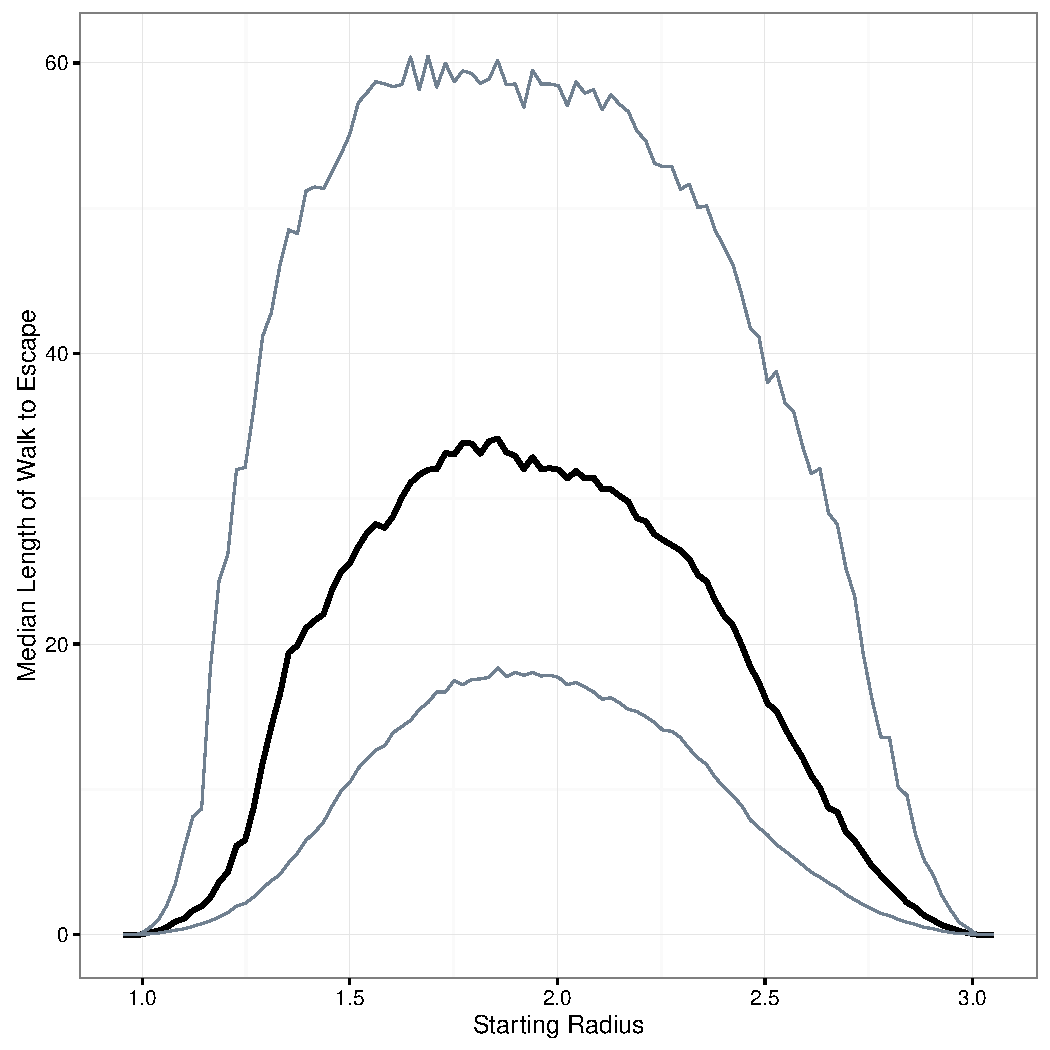
\includegraphics[width=0.85\textwidth]{images/PlaneIn1Out3.pdf}
	\end{figure}

\end{frame}

%---------------------------------------------------------------

\begin{frame}
	
	\frametitle{Plane}
	
	\begin{figure}
		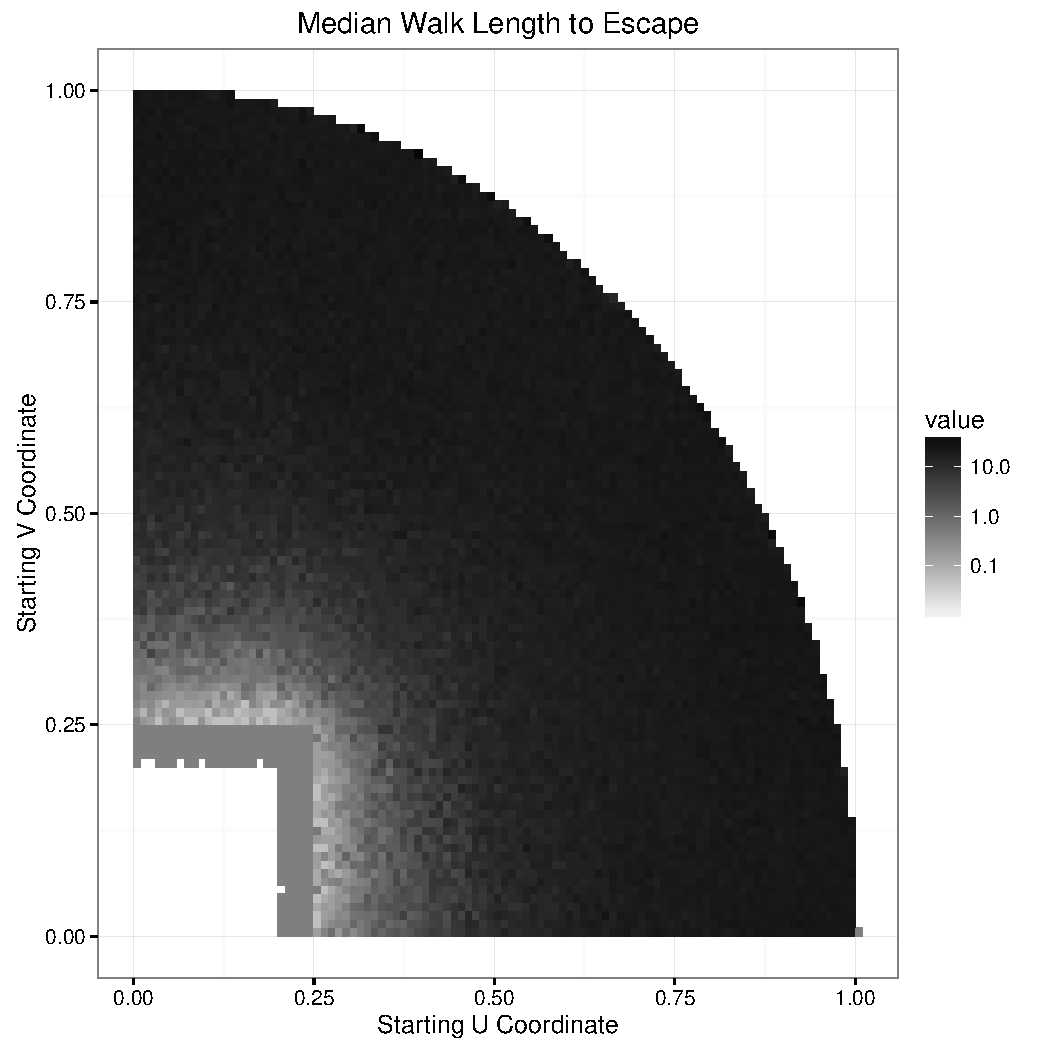
\includegraphics[width=0.85\textwidth]{images/PlaneCircleL05.pdf}
	\end{figure}
	
\end{frame}

%---------------------------------------------------------------

\begin{frame}
	
	\frametitle{Sphere}
	
	\begin{figure}
		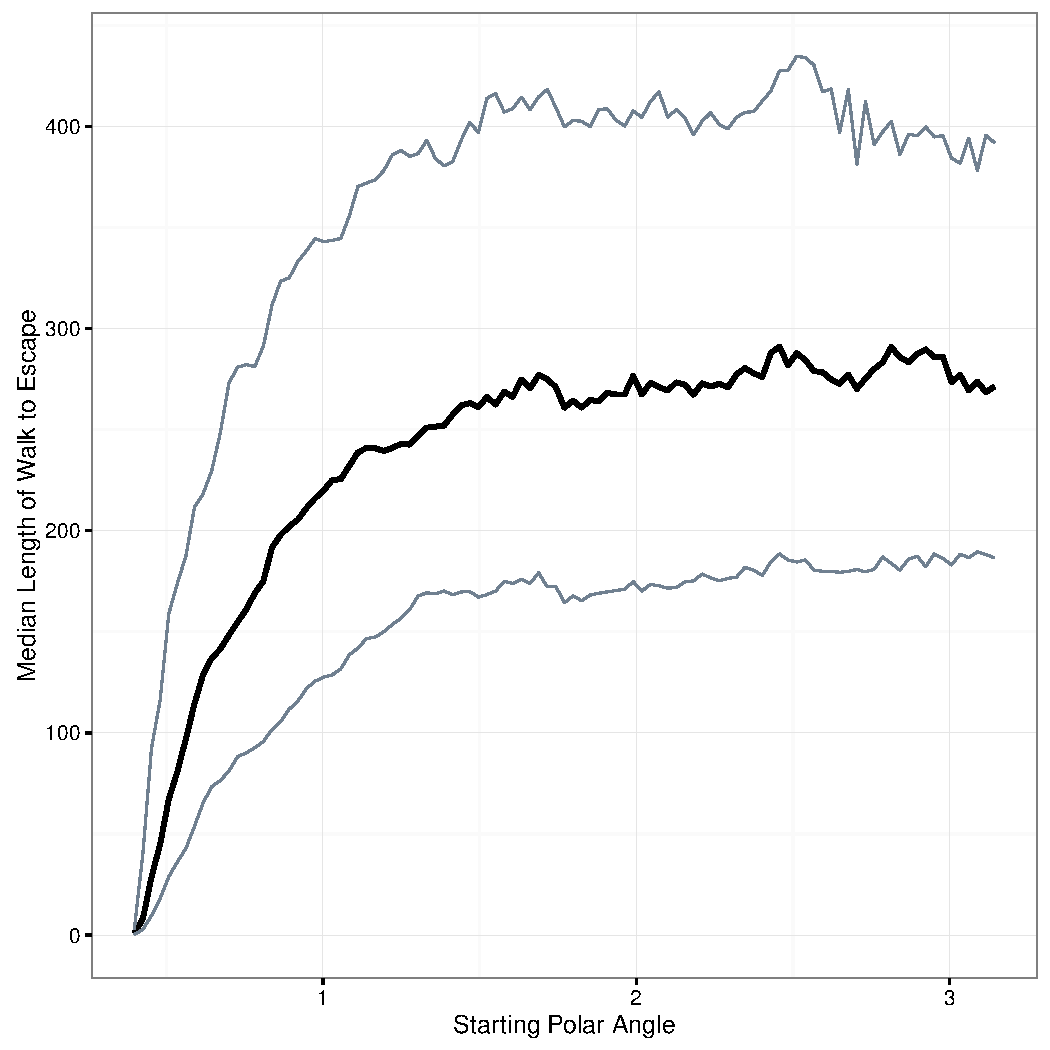
\includegraphics[width=0.85\textwidth]{images/ExampleSphereL04.pdf}
	\end{figure}
	
\end{frame}

%---------------------------------------------------------------

\begin{frame}
	
	\frametitle{Sphere}
	
	\begin{figure}
		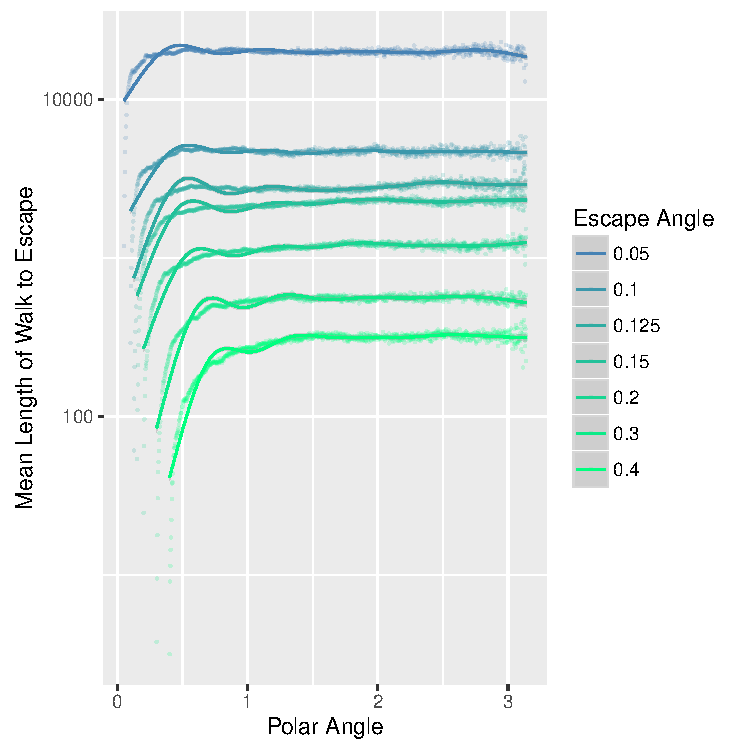
\includegraphics[width=0.85\textwidth]{images/SummaryPlot_L005_04.pdf}
	\end{figure}
	
\end{frame}

%---------------------------------------------------------------

\begin{frame}
	
	\frametitle{Torus}
	
	\begin{figure}
		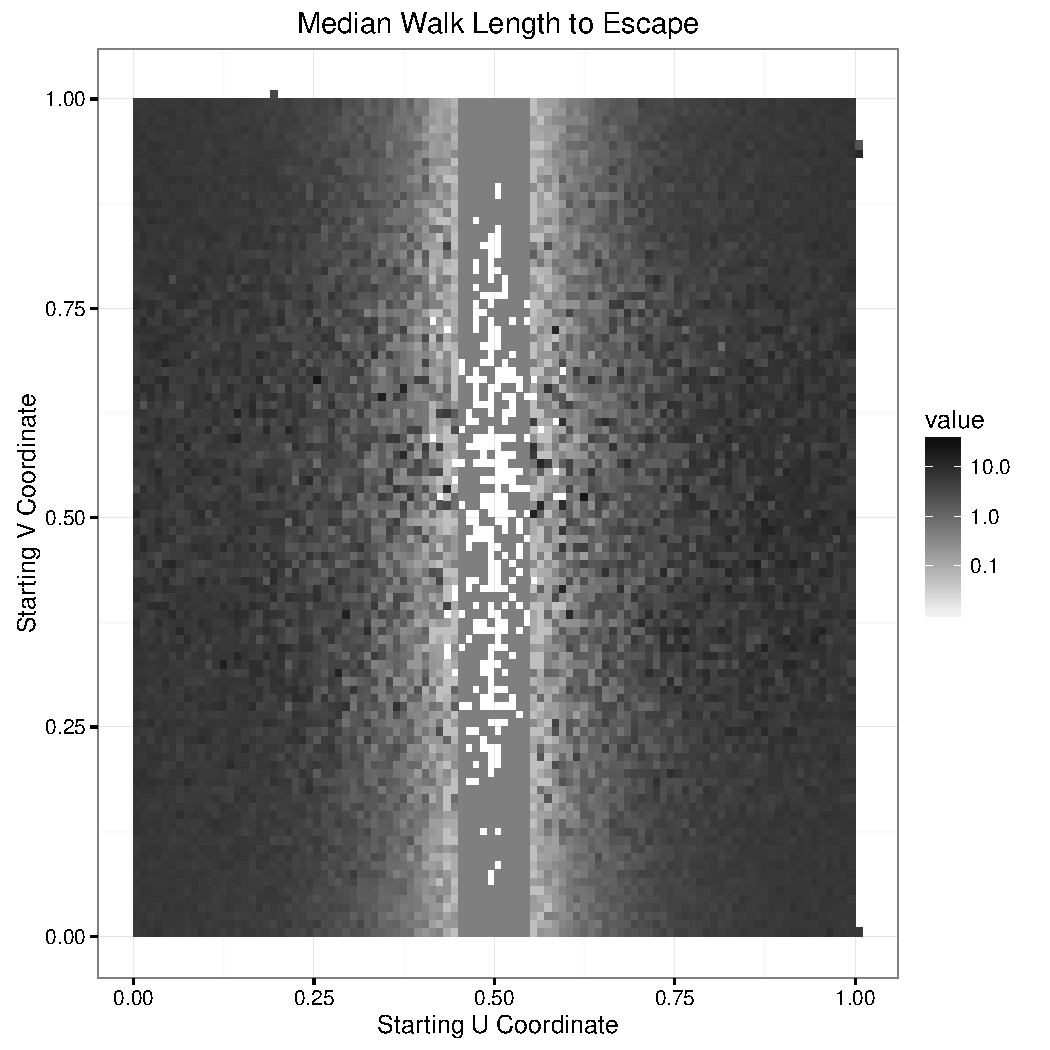
\includegraphics[width=0.85\textwidth]{images/TorusUBand.pdf}
	\end{figure}
	
\end{frame}
%---------------------------------------------------------------

\begin{frame}
	
	\frametitle{Torus}
	
	\begin{figure}
		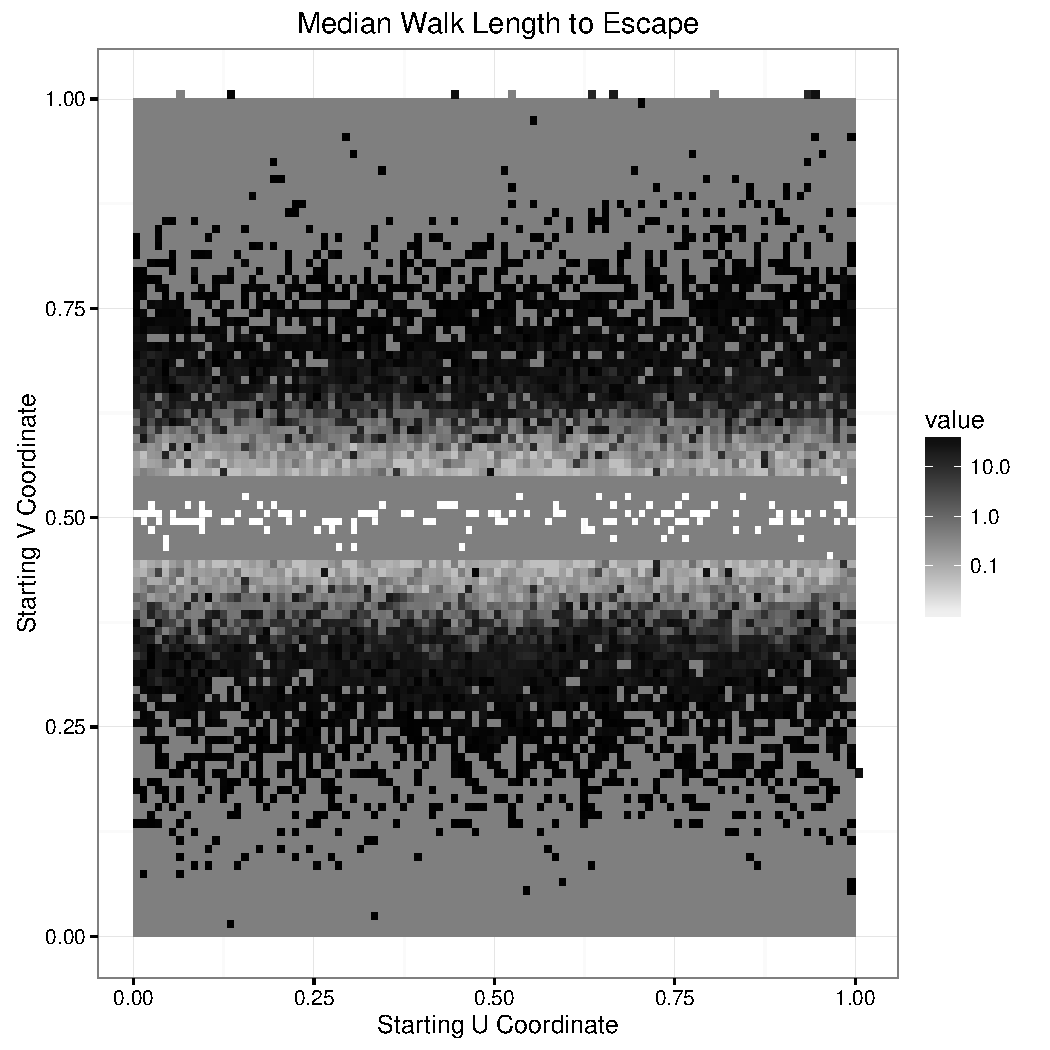
\includegraphics[width=0.85\textwidth]{images/TorusVBand.pdf}
	\end{figure}
	
\end{frame}

%---------------------------------------------------------------

\begin{frame}
	
	\frametitle{Overall Package}
	
	\begin{columns}
		\begin{column}{0.5\textwidth}
			\begin{itemize}
				\item Versatility
				\item Flexibility
				\item Speed
			\end{itemize}
		\end{column}
		
		\begin{column}{0.5\textwidth}
			\begin{itemize}
				\item Stepper
				\item Coordinate Wrappers
				\item Escape Checks
			\end{itemize}
		\end{column}
	\end{columns}
	
	
\end{frame}

%------------------------------------------------
\section{Questions}

\begin{frame}
\Huge{\centerline{Questions?}}
\end{frame}


\end{document} 